\chapter{Anexo 1. Criterios de selecci�n en �reas funcionales}

\begin{table}[H]
  \begin{figure}[H]
	\centering
	\fbox{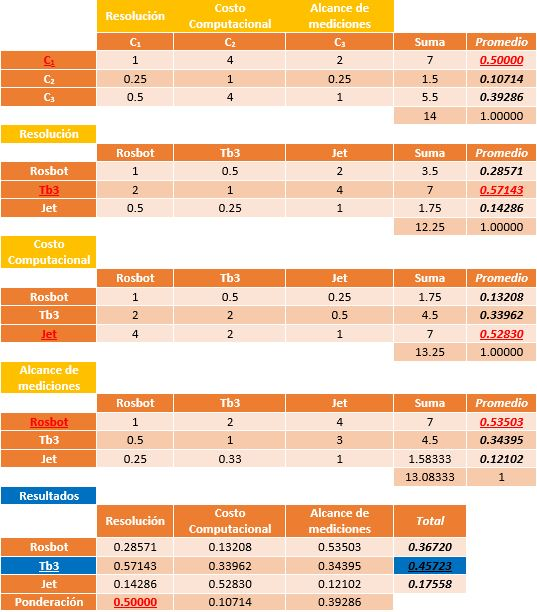
\includegraphics[scale=0.8]{imagenes/Anexos/01_Seleccion_Percepcion.jpg}}
  \end{figure}
    \caption{Tabla de selecci�n para Percepci�n}
    \label{tab:Tabla_percepcion}
\end{table}

\begin{table}[H]
 \begin{figure}[H]
	\centering
	\fbox{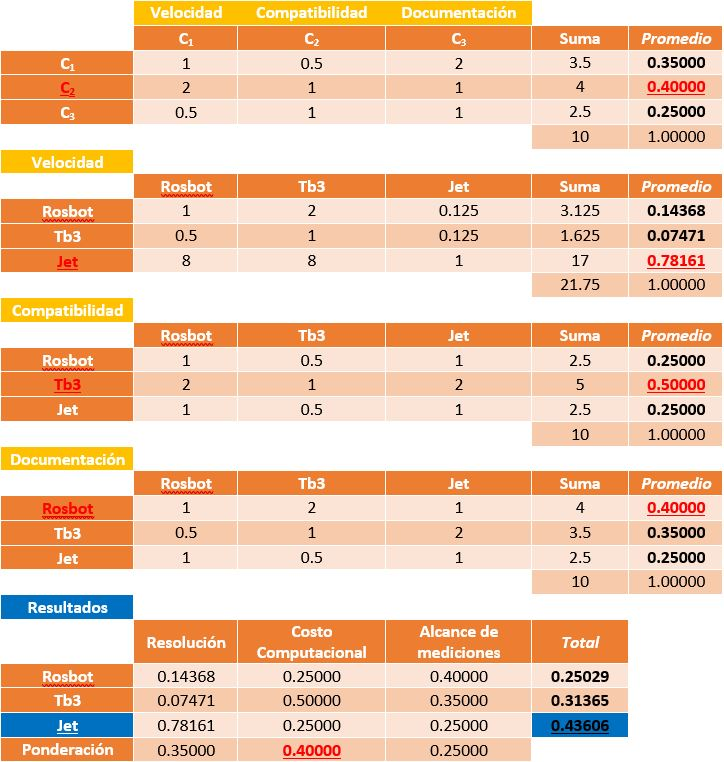
\includegraphics[scale=1]{imagenes/Anexos/02_Seleccion_Estructura.jpg}}
 \end{figure}
    \caption{Tabla de selecci�n para Estructura}
    \label{tab:Tabla_estructura}
\end{table}

\begin{table}[H]
 \begin{figure}[H]
	\centering
	\fbox{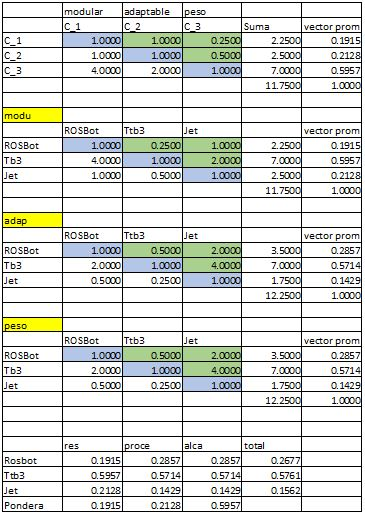
\includegraphics[scale=1]{imagenes/Anexos/03_Seleccion_Procesamiento.jpg}}
 \end{figure}
    \caption{Tabla de selecci�n para Procesamiento}
    \label{tab:Tabla_procesamiento}
\end{table}

\begin{table}[H]
	\begin{figure}[H]
		\centering
		\fbox{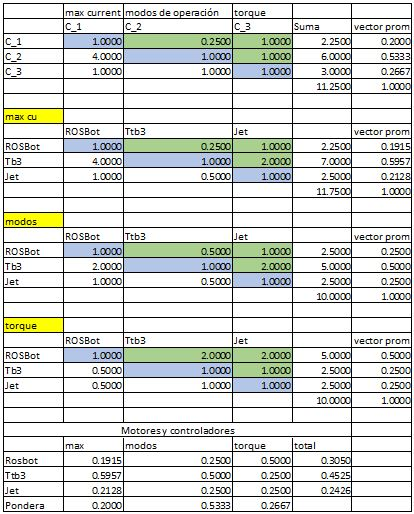
\includegraphics[scale=1]{imagenes/Anexos/04_Seleccion_Motores.jpg}}
	\end{figure}
	\caption{Tabla de selecci�n para Motores}
	\label{tab:Tabla_motores}
\end{table}